\section{Additional Functionality} \label{sec:additionalFunctionality}
\logToConsole{ADDITIONAL FUNCTIONALITY}

In this section, we describe additional functionality implemented in CORA.

% class reachset
\subsection{Class \texttt{reachSet}}
\label{sec:reachSet}

Reachable sets are stored as objects of class \texttt{reachSet}. This class implements several useful methods that make it very convenient to handle the resulting reachable sets.

An object of class \texttt{reachSet} can be constructed as follows:
\begin{equation*}
	\begin{split}
		& \texttt{R} = \texttt{reachSet}(\texttt{timePoint}), \\
		& \texttt{R} = \texttt{reachSet}(\texttt{timePoint},\texttt{parent}), \\
		& \texttt{R} = \texttt{reachSet}(\texttt{timePoint},\texttt{parent},\texttt{loc}), \\
		& \texttt{R} = \texttt{reachSet}(\texttt{timePoint},\texttt{timeInt}), \\
		& \texttt{R} = \texttt{reachSet}(\texttt{timePoint},\texttt{timeInt},\texttt{parent}), \\
		& \texttt{R} = \texttt{reachSet}(\texttt{timePoint},\texttt{timeInt},\texttt{parent},\texttt{loc}),
	\end{split}
\end{equation*}	
with input arguments
\begin{center}
\renewcommand{\arraystretch}{1.3}
\begin{tabular}[t]{l p{12cm} }
	$\bullet$~\texttt{timePoint} & struct with fields \texttt{.set} and \texttt{.time} storing reachable sets of time points.\\
	$\bullet$~\texttt{timeInt} & struct with fields \texttt{.set}, \texttt{.time}, and \texttt{.algebraic} (\texttt{nonlinDASys} only, see \cref{sec:nonlinearDASystems}) storing reachable sets of time intervals. \\
	$\bullet$~\texttt{parent} & index of the parent reachable set. \\
	$\bullet$~\texttt{loc} & index of the location (see \cref{sec:hybridDynamics}) to which the reachable set belongs (hybrid systems only).
\end{tabular}
\end{center}

The reachable set can consist of multiple strands as visualized in \cref{fig:reachSet}. New strands are created at location changes for hybrid systems, if reachable sets are split, and if reachable sets are united. For the reachable set shown in \cref{fig:reachSet}, the corresponding \texttt{reachSet} object is as follows:

\begin{center}
\begin{minipage}[t]{0.32\textwidth}
	\footnotesize
	\begin{verbatim}
		R = 

  5x1 reachSet array:

    timePoint
    timeInterval
    parent
    loc
	\end{verbatim}
\end{minipage}
\begin{minipage}[t]{0.32\textwidth}
	\footnotesize
	\begin{verbatim}
	R(1)

  reachSet with properties:

       timePoint: [1x1 struct]
    timeInterval: [1x1 struct]
          parent: 0
             loc: 1
	\end{verbatim}
\end{minipage}
\begin{minipage}[t]{0.32\textwidth}
	\footnotesize
	\begin{verbatim}
	R(2)

  reachSet with properties:

       timePoint: [1x1 struct]
    timeInterval: [1x1 struct]
          parent: 1
             loc: 2
	\end{verbatim}
\end{minipage}
\end{center}

\vspace{0.1cm}

\begin{center}
\begin{minipage}[t]{0.32\textwidth}
	\footnotesize
	\begin{verbatim}
	R(3)

  reachSet with properties:

       timePoint: [1x1 struct]
    timeInterval: [1x1 struct]
          parent: 2
             loc: 2
	\end{verbatim}
\end{minipage}
\begin{minipage}[t]{0.32\textwidth}
	\footnotesize
	\begin{verbatim}
	R(4)

  reachSet with properties:

       timePoint: [1x1 struct]
    timeInterval: [1x1 struct]
          parent: 2
             loc: 2
	\end{verbatim}
\end{minipage}
\begin{minipage}[t]{0.32\textwidth}
	\footnotesize
	\begin{verbatim}
	R(5)

  reachSet with properties:

       timePoint: [1x1 struct]
    timeInterval: [1x1 struct]
          parent: [3,4]
             loc: 2
	\end{verbatim}
\end{minipage}
\end{center}


\begin{figure}[htb]	
\begin{center}
	\includegraphics[width=0.7\columnwidth]{./figures/examples/example_reachSet.eps}	
	\caption{Example demonstrating the different strands of the reachable set.}
	\label{fig:reachSet}
	\end{center}
\end{figure}


%\newpage
Next, we explain the most common methods for the class \texttt{reachSet} in detail.



\subsubsection{\texttt{add}}

The method \texttt{add} adds a reachable set to another one:
\begin{equation*}
\begin{split}
	& \texttt{R} = \texttt{add}(\texttt{R1},\texttt{R2}), \\
	& \texttt{R} = \texttt{add}(\texttt{R1},\texttt{R2},\texttt{parent}),
\end{split}
\end{equation*}
where \texttt{R1} and \texttt{R2} are both objects of class \texttt{reachSet}, and \texttt{parent} is the index of the parent for the root element of \texttt{R2}. Adding reachable sets is for example useful if the overall reachable set is computed in multiple sequences.

\subsubsection{\texttt{find}}

The method \texttt{find} returns all reachable sets that satisfy the specified condition:
\begin{equation*}
	\texttt{res} = \texttt{find}(\texttt{R},\texttt{prop},\texttt{val}),
\end{equation*}
where \texttt{R} is an object of class \texttt{reachSet}, \texttt{prop} is a string specifying the property for the condition, \texttt{val} is the desired value of the property, and \texttt{res} is an object of class \texttt{reachSet} containing all reachable sets that satisfy the property.  Currently, the following values for \texttt{prop} are supported:
\begin{itemize}
	\item \texttt{'location'}: find all reachable sets that correspond to the specified location.
	\item \texttt{'parent'}: find all reachable sets with the specified parent.
	\item \texttt{'time'}: find all reachable sets that correspond to the specified time interval.
\end{itemize}


\subsubsection{\texttt{plot}}

The method \texttt{plot} visualizes a two-dimensional projection of the boundary of reachable set for time intervals:
%
\begin{align*}
	\begin{split}
		&\texttt{han} = \operator{plot}(\texttt{R}), \\
		&\texttt{han} = \operator{plot}(\texttt{R},\texttt{dim}), \\
		&\texttt{han} = \operator{plot}(\texttt{R},\texttt{dim},\texttt{linespec}), \\
		&\texttt{han} = \operator{plot}(\texttt{R},\texttt{dims},\texttt{linespec},\texttt{namevaluepairs}),
	\end{split}
\end{align*}
where \texttt{R} is an object of class \texttt{reachSet}, \texttt{han} is a handle to the plotted MATLAB graphics object, and the additional input arguments are defined as

\begin{itemize}
	\item \texttt{dims}: Integer vector $\texttt{dims} \in \mathbb{N}_{\leq n}^2$ specifying the dimensions for which the projection is visualized (default value: \texttt{dims = [1 2]}).
	\item \texttt{linespec}: (optional) line specifications, e.g., \texttt{'--*r'}, as supported by MATLAB\footnote{\url{https://de.mathworks.com/help/matlab/ref/linespec.html}}.
	\item \texttt{namevaluepairs}: (optional) further specifications as name-value pairs, e.g.,
	\texttt{'LineWidth',2} and \texttt{'FaceColor',[.5 .5 .5]}, as supported by MATLAB.
	If the plot is not filled, these are the built-in
	Line Properties\footnote{\url{https://de.mathworks.com/help/matlab/ref/matlab.graphics.chart.primitive.line-properties.html}},
	if the plot is filled, they correspond to the Patch Properties\footnote{\url{https://de.mathworks.com/help/matlab/ref/matlab.graphics.primitive.patch-properties.html}}.
\end{itemize}
%
The following name-value pairs enhance the built-in functionalities:
\begin{itemize}
	\item \texttt{'Order'}: zonotope order for plotting. If provided,
		the zonotope order is reduced to the given order before the set is plotted.
	\item \texttt{'Splits'}: number of splits applied to refine the plotted over-approximation
		of polynomial zonotopes (polynomial zonotopes only, see \cref{sec:polynomialZonotopes}).
	\item \texttt{'Unify'}: If the name-value pair \texttt{'Unify',true} is passed the union of all reachable sets is computed to avoid overlapping regions in the plot. The resulting figure then usually requires significantly less storage space. 
\end{itemize}

For discrete-time systems (see \cref{sec:linearSysDT} and \cref{sec:nonlinearSystemsDT}), the reachable set at time points is visualized since there exists no reachable set for time intervals.


\subsubsection{\texttt{plotOverTime}}

The method \texttt{plotOverTime} visualizes a one-dimensional projection of the reachable set of time intervals over time:
%
\begin{align*}
	\begin{split}
		&\texttt{han} = \operator{plotOverTime}(\texttt{R}), \\
		&\texttt{han} = \operator{plotOverTime}(\texttt{R},\texttt{dims}), \\
		&\texttt{han} = \operator{plotOverTime}(\texttt{R},\texttt{dims},\texttt{linespec}), \\
		&\texttt{han} = \operator{plotOverTime}(\texttt{R},\texttt{dims},\texttt{linespec},\texttt{namevaluepairs}),
	\end{split}
\end{align*}
where \texttt{R} is an object of class \texttt{reachSet}, \texttt{han} is a handle to the plotted MATLAB graphics object, and the additional input arguments are defined as

\begin{itemize}
	\item \texttt{dims}: Integer vector $\texttt{dims} \in \mathbb{N}_{\leq n}$ specifying the dimensions for which the projection is visualized (default value: \texttt{dim = 1}).
	\item \texttt{linespec}: (optional) line specifications, e.g., \texttt{'--*r'}, as supported by MATLAB\footnote{\url{https://de.mathworks.com/help/matlab/ref/linespec.html}}.
	\item \texttt{namevaluepairs}: (optional) further specifications as name-value pairs, e.g.,
	\texttt{'LineWidth',2} and \texttt{'FaceColor',[.5 .5 .5]}, as supported by MATLAB.
	They correspond to the Patch Properties\footnote{\url{https://de.mathworks.com/help/matlab/ref/matlab.graphics.primitive.patch-properties.html}}.
\end{itemize}
%
The following name-value pairs enhance the built-in functionalities:
\begin{itemize}	
	\item \texttt{'Unify'}: If the name-value pair \texttt{'Unify',true} is passed the union of all reachable sets is computed to avoid overlapping regions in the plot. The resulting figure then usually requires significantly less storage space. %especially useful when the reachable set has several strands 
\end{itemize}
For discrete-time systems (see \cref{sec:linearSysDT} and \cref{sec:nonlinearSystemsDT}), the reachable set at time points is visualized since there exists no reachable set for time intervals.


\subsubsection{query}

The method \texttt{query} returns the value of a certain property of an object of class \texttt{reachSet}:
\begin{equation*}
	\texttt{val} = \texttt{query}(\texttt{R},\texttt{prop}),
\end{equation*}
where \texttt{R} is an object of class \texttt{reachSet}, \texttt{prop} is a string specifying the property of interest, and \texttt{val} is the value of the property. Currently, the following values for \texttt{prop} are supported:
\begin{itemize}
	\item \texttt{'reachSet'}: returns all reachable sets of time intervals as a cell array.
	\item \texttt{'reachSetTimePoint'}: returns all reachable sets at points in time as a cell array.
	\item \texttt{'finalSet'}: returns the last time-point reachable set.
	\item \texttt{'tVec'}: returns the vector of time step sizes (only supported for one single strand).
\end{itemize}


% class simResult
\subsection{Class \texttt{simResult}}
\label{sec:simResult}

The results of simulations are stored in CORA as objects of the class \texttt{simResult}, which provides several methods to easily visualize the simulated trajectories. An object of class \texttt{simResult} can be constructed as follows:
\begin{equation*}
	\begin{split}
		& \texttt{simRes} = \texttt{simResult}(\texttt{x},\texttt{t}), \\
		& \texttt{simRes} = \texttt{simResult}(\texttt{x},\texttt{t},\texttt{loc}),
	\end{split}
\end{equation*}
with input arguments
\begin{center}
\renewcommand{\arraystretch}{1.3}
\begin{tabular}[t]{l p{13cm} }
	$\bullet$~\texttt{x} & cell array storing the states of the simulated trajectories.\\
	$\bullet$~\texttt{t} & cell array storing the time points for the simulated trajectories. \\
	$\bullet$~\texttt{loc} & cell array storing the indices of the locations for the simulated trajectories (hybrid systems only).
\end{tabular}
\end{center}

Next, we explain the methods of the class \texttt{simResult} in detail.

\subsubsection{\texttt{add}}

The method \texttt{add} combines two \texttt{simResult} objects \texttt{simRes1} and \texttt{simRes2}:
\begin{equation*}
	\texttt{simRes} = \texttt{add}(\texttt{simRes1},\texttt{simRes2}).
\end{equation*}


\subsubsection{\texttt{plot}}

The method \texttt{plot} visualizes a two-dimensional projection of the obtained trajectories:

\begin{equation*}
	\begin{split}
		&\texttt{han} = \operator{plot}(\texttt{simRes}), \\
		&\texttt{han} = \operator{plot}(\texttt{simRes},\texttt{dims}), \\
		&\texttt{han} = \operator{plot}(\texttt{simRes},\texttt{dims},\texttt{linespec}), \\
		&\texttt{han} = \operator{plot}(\texttt{simRes},\texttt{dims},\texttt{namevaluepairs}),
	\end{split}
\end{equation*}
where \texttt{simRes} is an object of class \texttt{simResult}, \texttt{han} is a handle to the plotted MATLAB graphics object, and the additional input arguments are defined as

\begin{itemize}
	\item \texttt{dims}: Integer vector $\texttt{dims} \in \mathbb{N}_{\leq n}^2$ specifying the dimensions for which the projection is visualized (default value: \texttt{dims = [1 2]}).
	\item \texttt{linespec}: (optional) line specifications, e.g., \texttt{'--*r'}, as supported by MATLAB\footnote{\url{https://de.mathworks.com/help/matlab/ref/linespec.html}} (default value: \texttt{linespec = 'b'}).
	\item \texttt{namevaluepairs}: (optional) further specifications as name-value pairs, e.g.,
	\texttt{'LineWidth',2} and \texttt{'MarkerSize',1.5}, as supported by MATLAB.
	They correspond to the Line Properties\footnote{\url{https://de.mathworks.com/help/matlab/ref/matlab.graphics.chart.primitive.line-properties.html}}.
\end{itemize}


\subsubsection{\texttt{plotOverTime}}

The method \texttt{plotOverTime} visualizes a one-dimensional projection of the simulated trajectories over time:

\begin{equation*}
	\begin{split}
		&\texttt{han} = \operator{plotOverTime}(\texttt{simRes}), \\
		&\texttt{han} = \operator{plotOverTime}(\texttt{simRes},\texttt{dims}), \\
		&\texttt{han} = \operator{plotOverTime}(\texttt{simRes},\texttt{dims},\texttt{linespec}), \\
		&\texttt{han} = \operator{plotOverTime}(\texttt{simRes},\texttt{dims},\texttt{namevaluepairs}),
	\end{split}
\end{equation*}
where \texttt{simRes} is an object of class \texttt{simResult}, \texttt{han} is a handle to the plotted MATLAB graphics object, and the additional input arguments are defined as

\begin{itemize}
	\item \texttt{dims}: Integer vector $\texttt{dims} \in \mathbb{N}_{\leq n}$ specifying the dimensions for which the projection is visualized (default value: \texttt{dims = 1}).
	\item \texttt{linespec}: (optional) line specifications, e.g., \texttt{'--*r'}, as supported by MATLAB\footnote{\url{https://de.mathworks.com/help/matlab/ref/linespec.html}}.
	\item \texttt{namevaluepairs}: (optional) further specifications as name-value pairs, e.g.,
	\texttt{'LineWidth',2} and \texttt{'MarkerSize',1.5}, as supported by MATLAB.
	They correspond to the Line Properties\footnote{\url{https://de.mathworks.com/help/matlab/ref/matlab.graphics.primitive.patch-properties.html}}.
\end{itemize}


% class specification
\subsection{Class \texttt{specification}}
\label{sec:specification}

The class \texttt{specification} allows one to define specifications that a system has to satisfy (see \cref{sec:reach}). If specifications are provided, reachability analysis terminates as soon as a specification is violated. An object of class \texttt{specification} can be constructed as follows (note that $\mathcal{S}$ can be replaced by \texttt{list}):
\begin{equation*}
	\begin{split}
		& \texttt{spec} = \texttt{specification}(\mathcal{S}), \\
		& \texttt{spec} = \texttt{specification}(\mathcal{S},\texttt{type}), \\
		& \texttt{spec} = \texttt{specification}(\mathcal{S},\texttt{location}), \\
		& \texttt{spec} = \texttt{specification}(\mathcal{S},\texttt{type},\texttt{location}), \\
		& \texttt{spec} = \texttt{specification}(\mathcal{S},\texttt{type},\texttt{time}), \\
		& \texttt{spec} = \texttt{specification}(\mathcal{S},\texttt{type},\texttt{location},\texttt{time}), \\
		& \texttt{spec} = \texttt{specification}(\mathcal{S},\texttt{type},\texttt{time},\texttt{location}), \\
		& \texttt{spec} = \texttt{specification}(\phi,\texttt{'logic'}), \\
     	& \texttt{spec} = \texttt{specification}(\texttt{func},\texttt{'custom'}), \\
		& \texttt{spec} = \texttt{specification}(\texttt{func},\texttt{'custom'},\texttt{time}), \\
		& \texttt{spec} = \texttt{specification}(\texttt{func},\texttt{'custom'},\texttt{location}), \\
		& \texttt{spec} = \texttt{specification}(\texttt{func},\texttt{'custom'},\texttt{time},\texttt{location}), \\
		& \texttt{spec} = \texttt{specification}(\texttt{func},\texttt{'custom'},\texttt{location},\texttt{time}),
	\end{split}
\end{equation*}
where the input arguments are defined as follows:

\begin{center}
\renewcommand{\arraystretch}{1.3}
\begin{tabular}[t]{l p{13cm} }
	$\bullet$~$\mathbf{\mathcal{S}}$ & set which defines the specification represented by one of the set representations in \cref{sec:setRepresentations}. \\
	$\bullet$~\textbf{\texttt{list}} & cell array storing the sets which define the specifications. Useful for constructing multiple specifications at once.\\
	$\bullet$~\textbf{\texttt{type}} & string specifying the type of the specifications. Supported types are \texttt{'unsafeSet'}, \texttt{'safeSet'}, \texttt{'invariant'}, and \texttt{'custom'}. \\
	$\bullet$~\textbf{\texttt{location}} & for hybrid automata (see \cref{sec:hybridAutomaton}): double array specifying in which location of a hybrid automaton the specification is active, can also be set to \texttt{[]} meaning active in all locations (default); for parallel hybrid automata (see \cref{sec:parallelHybridAutomata}): cell-array of double arrays specifying list of active locations for each component of the hybrid automaton \\
	$\bullet$~\textbf{\texttt{time}} & time interval in which the specification is valid specified as an object of class interval (see \cref{sec:interval}). The default value is the empty interval, which stands for valid at all times. \\
	$\bullet$~$\mathbf{\phi}$ & temporal logic specification represented as an object of class \texttt{stl} (see \cref{sec:temporalLogic}). \\
	$\bullet$~\textbf{\texttt{func}} & function handle to a function $f(\mathcal{R})$ that takes the current reachable set $\mathcal{R}$ for time intervals as an input argument and returns \texttt{true} if the custom specification is satisfied, and \texttt{false} otherwise.
\end{tabular}
\end{center}

Let us denote the reachable set at time $t$ as $\mathcal{R}(t)$. The different types of specifications are defined as follows:
\begin{align*}
	&\texttt{'unsafeSet'}: &\forall t \in [t_0,t_f]: ~ \mathcal{R}(t) \cap \mathcal{S} = \emptyset \\
	&\texttt{'safeSet'}: &\forall t \in [t_0,t_f]: ~ \mathcal{R}(t) \subseteq \mathcal{S} ~~~~~\\
	&\texttt{'invariant'}\footnotemark: &\forall t \in [t_0,t_f]: ~ \mathcal{R}(t) \cap \mathcal{S} \neq \emptyset \\
	&\texttt{'logic'}: &\forall \xi(t) \in \mathcal{R}(t): ~ \xi(t) \models \phi ~~~~\\
	&\texttt{'custom'}: &\forall t \in [t_0,t_f]: ~ f(\mathcal{R}(t)) = 1,
\end{align*}
\footnotetext{Please note that this specification does not check for invariants as defined in \cite{Blanchini1999}, but whether a reachable set is still within an invariant $\mathcal{S}$ as specified for hybrid systems.}%
where $t_0$ is the initial and $t_f$ the final time for the reachable set computation. It is also possible to combine mutliple specifications using the method \texttt{add} (see \cref{sec:specAdd}). Let us demonstrate the construction of a specification by an example:

\begin{center}
\begin{minipage}[t]{0.55\textwidth}
	\vspace{10pt}
	\footnotesize
	% This file was created by matlab2tikz.
%
\definecolor{mycolor1}{rgb}{0.47060,0.77250,0.49800}%
\definecolor{mycolor2}{rgb}{0.94510,0.55290,0.56860}%
%
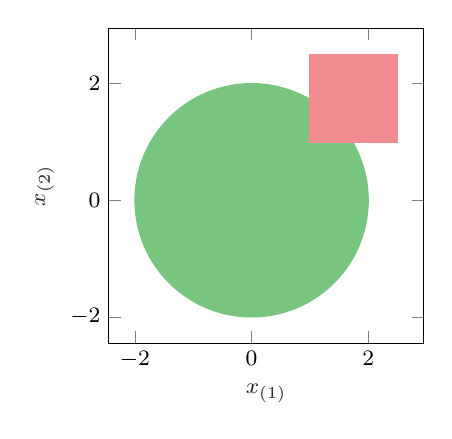
\begin{tikzpicture}
\footnotesize

\begin{axis}[%
width=4cm,
height=4cm,
at={(0in,0in)},
scale only axis,
xmin=-2.45,
xmax=2.95,
xlabel style={font=\color{white!15!black}},
xlabel={$x_{(1)}$},
ymin=-2.45,
ymax=2.95,
ylabel style={font=\color{white!15!black}},
ylabel={$x_{(2)}$},
axis background/.style={fill=white}
]

\addplot[area legend, draw=mycolor1, fill=mycolor1, forget plot]
table[row sep=crcr] {%
x	y\\
2	0.0063\\
1.9999	0.0188\\
1.9998	0.0314\\
1.9995	0.044\\
1.9992	0.0565\\
1.9988	0.0691\\
1.9983	0.0817\\
1.9978	0.0942\\
1.9971	0.1068\\
1.9964	0.1193\\
1.9956	0.1319\\
1.9948	0.1444\\
1.9928	0.1694\\
1.9917	0.182\\
1.9893	0.207\\
1.9865	0.232\\
1.985	0.2444\\
1.9818	0.2694\\
1.9782	0.2942\\
1.9763	0.3067\\
1.9744	0.3191\\
1.9702	0.3439\\
1.968	0.3562\\
1.9657	0.3686\\
1.9634	0.3809\\
1.961	0.3933\\
1.9584	0.4056\\
1.9559	0.4179\\
1.9532	0.4302\\
1.9505	0.4424\\
1.9476	0.4547\\
1.9418	0.4791\\
1.9356	0.5035\\
1.9324	0.5156\\
1.9291	0.5277\\
1.9258	0.5399\\
1.9223	0.5519\\
1.9188	0.564\\
1.9152	0.5761\\
1.9116	0.5881\\
1.9079	0.6001\\
1.904	0.6121\\
1.9002	0.624\\
1.8922	0.6478\\
1.8881	0.6597\\
1.8839	0.6716\\
1.8753	0.6952\\
1.8709	0.7069\\
1.8664	0.7187\\
1.8619	0.7304\\
1.8572	0.7421\\
1.8525	0.7537\\
1.8478	0.7654\\
1.8429	0.777\\
1.838	0.7885\\
1.833	0.8001\\
1.8279	0.8116\\
1.8228	0.823\\
1.8176	0.8345\\
1.8123	0.8459\\
1.807	0.8572\\
1.8015	0.8686\\
1.7961	0.8799\\
1.7905	0.8911\\
1.7849	0.9024\\
1.7792	0.9136\\
1.7734	0.9247\\
1.7675	0.9359\\
1.7616	0.9469\\
1.7556	0.958\\
1.7496	0.969\\
1.7435	0.98\\
1.7373	0.9909\\
1.7247	1.0127\\
1.7183	1.0235\\
1.7118	1.0343\\
1.7053	1.045\\
1.6987	1.0557\\
1.692	1.0663\\
1.6853	1.077\\
1.6785	1.0875\\
1.6647	1.1085\\
1.6577	1.119\\
1.6506	1.1294\\
1.6435	1.1397\\
1.6363	1.15\\
1.629	1.1603\\
1.6217	1.1705\\
1.6143	1.1806\\
1.6069	1.1908\\
1.5994	1.2008\\
1.5918	1.2109\\
1.5842	1.2208\\
1.5765	1.2308\\
1.5687	1.2407\\
1.5609	1.2505\\
1.553	1.2603\\
1.537	1.2797\\
1.5208	1.2989\\
1.5044	1.3179\\
1.4961	1.3273\\
1.4877	1.3367\\
1.4793	1.346\\
1.4708	1.3553\\
1.4536	1.3737\\
1.445	1.3828\\
1.4363	1.3918\\
1.4275	1.4008\\
1.4186	1.4098\\
1.4098	1.4186\\
1.4008	1.4275\\
1.3918	1.4363\\
1.3828	1.445\\
1.3737	1.4536\\
1.3553	1.4708\\
1.346	1.4793\\
1.3367	1.4877\\
1.3273	1.4961\\
1.3179	1.5044\\
1.2989	1.5208\\
1.2797	1.537\\
1.2603	1.553\\
1.2505	1.5609\\
1.2407	1.5687\\
1.2308	1.5765\\
1.2208	1.5842\\
1.2109	1.5918\\
1.2008	1.5994\\
1.1908	1.6069\\
1.1806	1.6143\\
1.1705	1.6217\\
1.1603	1.629\\
1.15	1.6363\\
1.1397	1.6435\\
1.1294	1.6506\\
1.119	1.6577\\
1.1085	1.6647\\
1.0875	1.6785\\
1.077	1.6853\\
1.0663	1.692\\
1.0557	1.6987\\
1.045	1.7053\\
1.0343	1.7118\\
1.0235	1.7183\\
1.0127	1.7247\\
0.9909	1.7373\\
0.98	1.7435\\
0.969	1.7496\\
0.958	1.7556\\
0.9469	1.7616\\
0.9359	1.7675\\
0.9247	1.7734\\
0.9136	1.7792\\
0.9024	1.7849\\
0.8911	1.7905\\
0.8799	1.7961\\
0.8686	1.8015\\
0.8572	1.807\\
0.8459	1.8123\\
0.8345	1.8176\\
0.823	1.8228\\
0.8116	1.8279\\
0.8001	1.833\\
0.7885	1.838\\
0.777	1.8429\\
0.7654	1.8478\\
0.7537	1.8525\\
0.7421	1.8572\\
0.7304	1.8619\\
0.7187	1.8664\\
0.7069	1.8709\\
0.6952	1.8753\\
0.6716	1.8839\\
0.6597	1.8881\\
0.6478	1.8922\\
0.624	1.9002\\
0.6121	1.904\\
0.6001	1.9079\\
0.5881	1.9116\\
0.5761	1.9152\\
0.564	1.9188\\
0.5519	1.9223\\
0.5399	1.9258\\
0.5277	1.9291\\
0.5156	1.9324\\
0.5035	1.9356\\
0.4791	1.9418\\
0.4547	1.9476\\
0.4424	1.9505\\
0.4302	1.9532\\
0.4179	1.9559\\
0.4056	1.9584\\
0.3933	1.961\\
0.3809	1.9634\\
0.3686	1.9657\\
0.3562	1.968\\
0.3439	1.9702\\
0.3191	1.9744\\
0.3067	1.9763\\
0.2942	1.9782\\
0.2694	1.9818\\
0.2444	1.985\\
0.232	1.9865\\
0.207	1.9893\\
0.182	1.9917\\
0.1694	1.9928\\
0.1444	1.9948\\
0.1319	1.9956\\
0.1193	1.9964\\
0.1068	1.9971\\
0.0942	1.9978\\
0.0817	1.9983\\
0.0691	1.9988\\
0.0565	1.9992\\
0.044	1.9995\\
0.0314	1.9998\\
0.0188	1.9999\\
0.0063	2\\
-0.0063	2\\
-0.0188	1.9999\\
-0.0314	1.9998\\
-0.044	1.9995\\
-0.0565	1.9992\\
-0.0691	1.9988\\
-0.0817	1.9983\\
-0.0942	1.9978\\
-0.1068	1.9971\\
-0.1193	1.9964\\
-0.1319	1.9956\\
-0.1444	1.9948\\
-0.1694	1.9928\\
-0.182	1.9917\\
-0.207	1.9893\\
-0.232	1.9865\\
-0.2444	1.985\\
-0.2694	1.9818\\
-0.2942	1.9782\\
-0.3067	1.9763\\
-0.3191	1.9744\\
-0.3439	1.9702\\
-0.3562	1.968\\
-0.3686	1.9657\\
-0.3809	1.9634\\
-0.3933	1.961\\
-0.4056	1.9584\\
-0.4179	1.9559\\
-0.4302	1.9532\\
-0.4424	1.9505\\
-0.4547	1.9476\\
-0.4791	1.9418\\
-0.5035	1.9356\\
-0.5156	1.9324\\
-0.5277	1.9291\\
-0.5399	1.9258\\
-0.5519	1.9223\\
-0.564	1.9188\\
-0.5761	1.9152\\
-0.5881	1.9116\\
-0.6001	1.9079\\
-0.6121	1.904\\
-0.624	1.9002\\
-0.6478	1.8922\\
-0.6597	1.8881\\
-0.6716	1.8839\\
-0.6952	1.8753\\
-0.7069	1.8709\\
-0.7187	1.8664\\
-0.7304	1.8619\\
-0.7421	1.8572\\
-0.7537	1.8525\\
-0.7654	1.8478\\
-0.777	1.8429\\
-0.7885	1.838\\
-0.8001	1.833\\
-0.8116	1.8279\\
-0.823	1.8228\\
-0.8345	1.8176\\
-0.8459	1.8123\\
-0.8572	1.807\\
-0.8686	1.8015\\
-0.8799	1.7961\\
-0.8911	1.7905\\
-0.9024	1.7849\\
-0.9136	1.7792\\
-0.9247	1.7734\\
-0.9359	1.7675\\
-0.9469	1.7616\\
-0.958	1.7556\\
-0.969	1.7496\\
-0.98	1.7435\\
-0.9909	1.7373\\
-1.0127	1.7247\\
-1.0235	1.7183\\
-1.0343	1.7118\\
-1.045	1.7053\\
-1.0557	1.6987\\
-1.0663	1.692\\
-1.077	1.6853\\
-1.0875	1.6785\\
-1.1085	1.6647\\
-1.119	1.6577\\
-1.1294	1.6506\\
-1.1397	1.6435\\
-1.15	1.6363\\
-1.1603	1.629\\
-1.1705	1.6217\\
-1.1806	1.6143\\
-1.1908	1.6069\\
-1.2008	1.5994\\
-1.2109	1.5918\\
-1.2208	1.5842\\
-1.2308	1.5765\\
-1.2407	1.5687\\
-1.2505	1.5609\\
-1.2603	1.553\\
-1.2797	1.537\\
-1.2989	1.5208\\
-1.3179	1.5044\\
-1.3273	1.4961\\
-1.3367	1.4877\\
-1.346	1.4793\\
-1.3553	1.4708\\
-1.3737	1.4536\\
-1.3828	1.445\\
-1.3918	1.4363\\
-1.4008	1.4275\\
-1.4098	1.4186\\
-1.4186	1.4098\\
-1.4275	1.4008\\
-1.4363	1.3918\\
-1.445	1.3828\\
-1.4536	1.3737\\
-1.4708	1.3553\\
-1.4793	1.346\\
-1.4877	1.3367\\
-1.4961	1.3273\\
-1.5044	1.3179\\
-1.5208	1.2989\\
-1.537	1.2797\\
-1.553	1.2603\\
-1.5609	1.2505\\
-1.5687	1.2407\\
-1.5765	1.2308\\
-1.5842	1.2208\\
-1.5918	1.2109\\
-1.5994	1.2008\\
-1.6069	1.1908\\
-1.6143	1.1806\\
-1.6217	1.1705\\
-1.629	1.1603\\
-1.6363	1.15\\
-1.6435	1.1397\\
-1.6506	1.1294\\
-1.6577	1.119\\
-1.6647	1.1085\\
-1.6785	1.0875\\
-1.6853	1.077\\
-1.692	1.0663\\
-1.6987	1.0557\\
-1.7053	1.045\\
-1.7118	1.0343\\
-1.7183	1.0235\\
-1.7247	1.0127\\
-1.7373	0.9909\\
-1.7435	0.98\\
-1.7496	0.969\\
-1.7556	0.958\\
-1.7616	0.9469\\
-1.7675	0.9359\\
-1.7734	0.9247\\
-1.7792	0.9136\\
-1.7849	0.9024\\
-1.7905	0.8911\\
-1.7961	0.8799\\
-1.8015	0.8686\\
-1.807	0.8572\\
-1.8123	0.8459\\
-1.8176	0.8345\\
-1.8228	0.823\\
-1.8279	0.8116\\
-1.833	0.8001\\
-1.838	0.7885\\
-1.8429	0.777\\
-1.8478	0.7654\\
-1.8525	0.7537\\
-1.8572	0.7421\\
-1.8619	0.7304\\
-1.8664	0.7187\\
-1.8709	0.7069\\
-1.8753	0.6952\\
-1.8839	0.6716\\
-1.8881	0.6597\\
-1.8922	0.6478\\
-1.9002	0.624\\
-1.904	0.6121\\
-1.9079	0.6001\\
-1.9116	0.5881\\
-1.9152	0.5761\\
-1.9188	0.564\\
-1.9223	0.5519\\
-1.9258	0.5399\\
-1.9291	0.5277\\
-1.9324	0.5156\\
-1.9356	0.5035\\
-1.9418	0.4791\\
-1.9476	0.4547\\
-1.9505	0.4424\\
-1.9532	0.4302\\
-1.9559	0.4179\\
-1.9584	0.4056\\
-1.961	0.3933\\
-1.9634	0.3809\\
-1.9657	0.3686\\
-1.968	0.3562\\
-1.9702	0.3439\\
-1.9744	0.3191\\
-1.9763	0.3067\\
-1.9782	0.2942\\
-1.9818	0.2694\\
-1.985	0.2444\\
-1.9865	0.232\\
-1.9893	0.207\\
-1.9917	0.182\\
-1.9928	0.1694\\
-1.9948	0.1444\\
-1.9956	0.1319\\
-1.9964	0.1193\\
-1.9971	0.1068\\
-1.9978	0.0942\\
-1.9983	0.0817\\
-1.9988	0.0691\\
-1.9992	0.0565\\
-1.9995	0.044\\
-1.9998	0.0314\\
-1.9999	0.0188\\
-2	0.0063\\
-2	-0.0063\\
-1.9999	-0.0188\\
-1.9998	-0.0314\\
-1.9995	-0.044\\
-1.9992	-0.0565\\
-1.9988	-0.0691\\
-1.9983	-0.0817\\
-1.9978	-0.0942\\
-1.9971	-0.1068\\
-1.9964	-0.1193\\
-1.9956	-0.1319\\
-1.9948	-0.1444\\
-1.9928	-0.1694\\
-1.9917	-0.182\\
-1.9893	-0.207\\
-1.9865	-0.232\\
-1.985	-0.2444\\
-1.9818	-0.2694\\
-1.9782	-0.2942\\
-1.9763	-0.3067\\
-1.9744	-0.3191\\
-1.9702	-0.3439\\
-1.968	-0.3562\\
-1.9657	-0.3686\\
-1.9634	-0.3809\\
-1.961	-0.3933\\
-1.9584	-0.4056\\
-1.9559	-0.4179\\
-1.9532	-0.4302\\
-1.9505	-0.4424\\
-1.9476	-0.4547\\
-1.9418	-0.4791\\
-1.9356	-0.5035\\
-1.9324	-0.5156\\
-1.9291	-0.5277\\
-1.9258	-0.5399\\
-1.9223	-0.5519\\
-1.9188	-0.564\\
-1.9152	-0.5761\\
-1.9116	-0.5881\\
-1.9079	-0.6001\\
-1.904	-0.6121\\
-1.9002	-0.624\\
-1.8922	-0.6478\\
-1.8881	-0.6597\\
-1.8839	-0.6716\\
-1.8753	-0.6952\\
-1.8709	-0.7069\\
-1.8664	-0.7187\\
-1.8619	-0.7304\\
-1.8572	-0.7421\\
-1.8525	-0.7537\\
-1.8478	-0.7654\\
-1.8429	-0.777\\
-1.838	-0.7885\\
-1.833	-0.8001\\
-1.8279	-0.8116\\
-1.8228	-0.823\\
-1.8176	-0.8345\\
-1.8123	-0.8459\\
-1.807	-0.8572\\
-1.8015	-0.8686\\
-1.7961	-0.8799\\
-1.7905	-0.8911\\
-1.7849	-0.9024\\
-1.7792	-0.9136\\
-1.7734	-0.9247\\
-1.7675	-0.9359\\
-1.7616	-0.9469\\
-1.7556	-0.958\\
-1.7496	-0.969\\
-1.7435	-0.98\\
-1.7373	-0.9909\\
-1.7247	-1.0127\\
-1.7183	-1.0235\\
-1.7118	-1.0343\\
-1.7053	-1.045\\
-1.6987	-1.0557\\
-1.692	-1.0663\\
-1.6853	-1.077\\
-1.6785	-1.0875\\
-1.6647	-1.1085\\
-1.6577	-1.119\\
-1.6506	-1.1294\\
-1.6435	-1.1397\\
-1.6363	-1.15\\
-1.629	-1.1603\\
-1.6217	-1.1705\\
-1.6143	-1.1806\\
-1.6069	-1.1908\\
-1.5994	-1.2008\\
-1.5918	-1.2109\\
-1.5842	-1.2208\\
-1.5765	-1.2308\\
-1.5687	-1.2407\\
-1.5609	-1.2505\\
-1.553	-1.2603\\
-1.537	-1.2797\\
-1.5208	-1.2989\\
-1.5044	-1.3179\\
-1.4961	-1.3273\\
-1.4877	-1.3367\\
-1.4793	-1.346\\
-1.4708	-1.3553\\
-1.4536	-1.3737\\
-1.445	-1.3828\\
-1.4363	-1.3918\\
-1.4275	-1.4008\\
-1.4186	-1.4098\\
-1.4098	-1.4186\\
-1.4008	-1.4275\\
-1.3918	-1.4363\\
-1.3828	-1.445\\
-1.3737	-1.4536\\
-1.3553	-1.4708\\
-1.346	-1.4793\\
-1.3367	-1.4877\\
-1.3273	-1.4961\\
-1.3179	-1.5044\\
-1.2989	-1.5208\\
-1.2797	-1.537\\
-1.2603	-1.553\\
-1.2505	-1.5609\\
-1.2407	-1.5687\\
-1.2308	-1.5765\\
-1.2208	-1.5842\\
-1.2109	-1.5918\\
-1.2008	-1.5994\\
-1.1908	-1.6069\\
-1.1806	-1.6143\\
-1.1705	-1.6217\\
-1.1603	-1.629\\
-1.15	-1.6363\\
-1.1397	-1.6435\\
-1.1294	-1.6506\\
-1.119	-1.6577\\
-1.1085	-1.6647\\
-1.0875	-1.6785\\
-1.077	-1.6853\\
-1.0663	-1.692\\
-1.0557	-1.6987\\
-1.045	-1.7053\\
-1.0343	-1.7118\\
-1.0235	-1.7183\\
-1.0127	-1.7247\\
-0.9909	-1.7373\\
-0.98	-1.7435\\
-0.969	-1.7496\\
-0.958	-1.7556\\
-0.9469	-1.7616\\
-0.9359	-1.7675\\
-0.9247	-1.7734\\
-0.9136	-1.7792\\
-0.9024	-1.7849\\
-0.8911	-1.7905\\
-0.8799	-1.7961\\
-0.8686	-1.8015\\
-0.8572	-1.807\\
-0.8459	-1.8123\\
-0.8345	-1.8176\\
-0.823	-1.8228\\
-0.8116	-1.8279\\
-0.8001	-1.833\\
-0.7885	-1.838\\
-0.777	-1.8429\\
-0.7654	-1.8478\\
-0.7537	-1.8525\\
-0.7421	-1.8572\\
-0.7304	-1.8619\\
-0.7187	-1.8664\\
-0.7069	-1.8709\\
-0.6952	-1.8753\\
-0.6716	-1.8839\\
-0.6597	-1.8881\\
-0.6478	-1.8922\\
-0.624	-1.9002\\
-0.6121	-1.904\\
-0.6001	-1.9079\\
-0.5881	-1.9116\\
-0.5761	-1.9152\\
-0.564	-1.9188\\
-0.5519	-1.9223\\
-0.5399	-1.9258\\
-0.5277	-1.9291\\
-0.5156	-1.9324\\
-0.5035	-1.9356\\
-0.4791	-1.9418\\
-0.4547	-1.9476\\
-0.4424	-1.9505\\
-0.4302	-1.9532\\
-0.4179	-1.9559\\
-0.4056	-1.9584\\
-0.3933	-1.961\\
-0.3809	-1.9634\\
-0.3686	-1.9657\\
-0.3562	-1.968\\
-0.3439	-1.9702\\
-0.3191	-1.9744\\
-0.3067	-1.9763\\
-0.2942	-1.9782\\
-0.2694	-1.9818\\
-0.2444	-1.985\\
-0.232	-1.9865\\
-0.207	-1.9893\\
-0.182	-1.9917\\
-0.1694	-1.9928\\
-0.1444	-1.9948\\
-0.1319	-1.9956\\
-0.1193	-1.9964\\
-0.1068	-1.9971\\
-0.0942	-1.9978\\
-0.0817	-1.9983\\
-0.0691	-1.9988\\
-0.0565	-1.9992\\
-0.044	-1.9995\\
-0.0314	-1.9998\\
-0.0188	-1.9999\\
-0.0063	-2\\
0.0063	-2\\
0.0188	-1.9999\\
0.0314	-1.9998\\
0.044	-1.9995\\
0.0565	-1.9992\\
0.0691	-1.9988\\
0.0817	-1.9983\\
0.0942	-1.9978\\
0.1068	-1.9971\\
0.1193	-1.9964\\
0.1319	-1.9956\\
0.1444	-1.9948\\
0.1694	-1.9928\\
0.182	-1.9917\\
0.207	-1.9893\\
0.232	-1.9865\\
0.2444	-1.985\\
0.2694	-1.9818\\
0.2942	-1.9782\\
0.3067	-1.9763\\
0.3191	-1.9744\\
0.3439	-1.9702\\
0.3562	-1.968\\
0.3686	-1.9657\\
0.3809	-1.9634\\
0.3933	-1.961\\
0.4056	-1.9584\\
0.4179	-1.9559\\
0.4302	-1.9532\\
0.4424	-1.9505\\
0.4547	-1.9476\\
0.4791	-1.9418\\
0.5035	-1.9356\\
0.5156	-1.9324\\
0.5277	-1.9291\\
0.5399	-1.9258\\
0.5519	-1.9223\\
0.564	-1.9188\\
0.5761	-1.9152\\
0.5881	-1.9116\\
0.6001	-1.9079\\
0.6121	-1.904\\
0.624	-1.9002\\
0.6478	-1.8922\\
0.6597	-1.8881\\
0.6716	-1.8839\\
0.6952	-1.8753\\
0.7069	-1.8709\\
0.7187	-1.8664\\
0.7304	-1.8619\\
0.7421	-1.8572\\
0.7537	-1.8525\\
0.7654	-1.8478\\
0.777	-1.8429\\
0.7885	-1.838\\
0.8001	-1.833\\
0.8116	-1.8279\\
0.823	-1.8228\\
0.8345	-1.8176\\
0.8459	-1.8123\\
0.8572	-1.807\\
0.8686	-1.8015\\
0.8799	-1.7961\\
0.8911	-1.7905\\
0.9024	-1.7849\\
0.9136	-1.7792\\
0.9247	-1.7734\\
0.9359	-1.7675\\
0.9469	-1.7616\\
0.958	-1.7556\\
0.969	-1.7496\\
0.98	-1.7435\\
0.9909	-1.7373\\
1.0127	-1.7247\\
1.0235	-1.7183\\
1.0343	-1.7118\\
1.045	-1.7053\\
1.0557	-1.6987\\
1.0663	-1.692\\
1.077	-1.6853\\
1.0875	-1.6785\\
1.1085	-1.6647\\
1.119	-1.6577\\
1.1294	-1.6506\\
1.1397	-1.6435\\
1.15	-1.6363\\
1.1603	-1.629\\
1.1705	-1.6217\\
1.1806	-1.6143\\
1.1908	-1.6069\\
1.2008	-1.5994\\
1.2109	-1.5918\\
1.2208	-1.5842\\
1.2308	-1.5765\\
1.2407	-1.5687\\
1.2505	-1.5609\\
1.2603	-1.553\\
1.2797	-1.537\\
1.2989	-1.5208\\
1.3179	-1.5044\\
1.3273	-1.4961\\
1.3367	-1.4877\\
1.346	-1.4793\\
1.3553	-1.4708\\
1.3737	-1.4536\\
1.3828	-1.445\\
1.3918	-1.4363\\
1.4008	-1.4275\\
1.4098	-1.4186\\
1.4186	-1.4098\\
1.4275	-1.4008\\
1.4363	-1.3918\\
1.445	-1.3828\\
1.4536	-1.3737\\
1.4708	-1.3553\\
1.4793	-1.346\\
1.4877	-1.3367\\
1.4961	-1.3273\\
1.5044	-1.3179\\
1.5208	-1.2989\\
1.537	-1.2797\\
1.553	-1.2603\\
1.5609	-1.2505\\
1.5687	-1.2407\\
1.5765	-1.2308\\
1.5842	-1.2208\\
1.5918	-1.2109\\
1.5994	-1.2008\\
1.6069	-1.1908\\
1.6143	-1.1806\\
1.6217	-1.1705\\
1.629	-1.1603\\
1.6363	-1.15\\
1.6435	-1.1397\\
1.6506	-1.1294\\
1.6577	-1.119\\
1.6647	-1.1085\\
1.6785	-1.0875\\
1.6853	-1.077\\
1.692	-1.0663\\
1.6987	-1.0557\\
1.7053	-1.045\\
1.7118	-1.0343\\
1.7183	-1.0235\\
1.7247	-1.0127\\
1.7373	-0.9909\\
1.7435	-0.98\\
1.7496	-0.969\\
1.7556	-0.958\\
1.7616	-0.9469\\
1.7675	-0.9359\\
1.7734	-0.9247\\
1.7792	-0.9136\\
1.7849	-0.9024\\
1.7905	-0.8911\\
1.7961	-0.8799\\
1.8015	-0.8686\\
1.807	-0.8572\\
1.8123	-0.8459\\
1.8176	-0.8345\\
1.8228	-0.823\\
1.8279	-0.8116\\
1.833	-0.8001\\
1.838	-0.7885\\
1.8429	-0.777\\
1.8478	-0.7654\\
1.8525	-0.7537\\
1.8572	-0.7421\\
1.8619	-0.7304\\
1.8664	-0.7187\\
1.8709	-0.7069\\
1.8753	-0.6952\\
1.8839	-0.6716\\
1.8881	-0.6597\\
1.8922	-0.6478\\
1.9002	-0.624\\
1.904	-0.6121\\
1.9079	-0.6001\\
1.9116	-0.5881\\
1.9152	-0.5761\\
1.9188	-0.564\\
1.9223	-0.5519\\
1.9258	-0.5399\\
1.9291	-0.5277\\
1.9324	-0.5156\\
1.9356	-0.5035\\
1.9418	-0.4791\\
1.9476	-0.4547\\
1.9505	-0.4424\\
1.9532	-0.4302\\
1.9559	-0.4179\\
1.9584	-0.4056\\
1.961	-0.3933\\
1.9634	-0.3809\\
1.9657	-0.3686\\
1.968	-0.3562\\
1.9702	-0.3439\\
1.9744	-0.3191\\
1.9763	-0.3067\\
1.9782	-0.2942\\
1.9818	-0.2694\\
1.985	-0.2444\\
1.9865	-0.232\\
1.9893	-0.207\\
1.9917	-0.182\\
1.9928	-0.1694\\
1.9948	-0.1444\\
1.9956	-0.1319\\
1.9964	-0.1193\\
1.9971	-0.1068\\
1.9978	-0.0942\\
1.9983	-0.0817\\
1.9988	-0.0691\\
1.9992	-0.0565\\
1.9995	-0.044\\
1.9998	-0.0314\\
1.9999	-0.0188\\
2	-0.0063\\
2	0.0063\\
}--cycle;

\addplot[area legend, draw=mycolor2, fill=mycolor2, forget plot]
table[row sep=crcr] {%
x	y\\
1	1\\
2.5	1\\
2.5	2.5\\
1	2.5\\
1	1\\
}--cycle;
\end{axis}
\end{tikzpicture}%
\end{minipage}
\begin{minipage}[t]{0.3\textwidth}
	\vspace{0pt}
	\centering
	\includetikz{./figures/tikz/add-functionality/example_specification}
\end{minipage}
\end{center}

Next, we explain the methods of class \texttt{specification} in detail.

\subsubsection{add}
\label{sec:specAdd}

The method \texttt{add} unites two specifications:
\begin{equation*}
	\texttt{spec} = \texttt{add}(\texttt{spec1},\texttt{spec2}),
\end{equation*}
where \texttt{spec1} and \texttt{spec2} are both objects of class \texttt{specification}. The specifications defined by \texttt{spec1} and \texttt{spec2} both have to be satisfied for the resulting specification \texttt{spec} to be satisfied.

\subsubsection{check}

The method \texttt{check} checks if a set $\mathcal{S} \subset \Rn$ satisfies the specification defined by the object \texttt{spec} of class \texttt{specification}:

\begin{equation*}
	\texttt{res} = \texttt{check}(\texttt{spec},\mathcal{S}),
\end{equation*}
where \texttt{res} is \texttt{true} if the specification is satisfied, and \texttt{false} otherwise.


% restructuring polynomial zonotopes
\subsection{Restructuring Polynomial Zonotopes}
\label{sec:restructurepolyZonotope}

In this subsection, we describe the settings for triggering and implementing the \texttt{restructure} operation of polynomial zonotopes (see \cref{sec:polynomialZonotopes}). As described in \cref{sec:nonlinearReach}, it is advantageous to use a non-convex set representation such as polynomial zonotopes to represent the reachable sets of nonlinear systems. Since during reachability analysis the size of the independent part of the polynomial zonotope constantly grows, the accuracy can be significantly improved by shifting generators from the independent to the dependent part as done by the \texttt{restructure} operation described in \cite[Sec.~2.5]{Kochdumper2021a}. For this restructuring process, there exist some additional settings listed in \cref{tab:polyZono}.

\begin{table}
\centering
\renewcommand{\arraystretch}{1.3}
\caption{Fields of the struct \texttt{options.polyZono} defining the settings for restructuring polynomial zonotopes (see \cite[Sec.~2.5]{Kochdumper2021a}).}
\label{tab:polyZono}
\begin{tabular}{ l p{11cm} }	
\toprule
\textbf{Setting} & \textbf{Description} \\
\midrule
	--~\texttt{.maxPolyZonoRatio} & upper bound $\mu_d$ for the volume ratio between the independent and dependent part of a polynomial zonotope (see \cite[Line~18 in Alg.~1]{Kochdumper2021a}). If the bound is exceeded, the polynomial zonotope is restructured. The default value is $\infty$ (no restructuring).  \\
	--~\texttt{.maxDepGenOrder} & upper bound for the value $\frac{p}{n}$ after restructuring, where $p$ is the number of dependent polynomial zonotope factors (see \cref{sec:polynomialZonotopes}) and $n$ is the system dimension. The default value is 20. \\
	--~\texttt{.restructureTechnique} & string specifying the method that is applied to restructure polynomial zonotopes. The string is composed of two parts \texttt{restructureTechnique} = \texttt{method} + \texttt{reductionTechnique}, where \texttt{method} represents the restructure strategy (see \cref{tab:restructureStrategy}) and \texttt{reductionTechnique} represents the zonotope reduction technique (see \cref{tab:zono_reduction}). Note that the two parts are combined by camelCase. The default value is \texttt{'reduceGirard'}. \\
\bottomrule
\end{tabular}
\end{table}


\begin{table}
\centering
\caption{Strategies for restructuring polynomial zonotopes}
\label{tab:restructureStrategy}
\begin{tabular}{ l l }	
\toprule
\textbf{Strategy} & \textbf{Description} \\
\midrule
\texttt{reduce} & reduction of independent generators \\
\texttt{reduceFull} & reduction of independent generators to zonotope order 1 \\
\texttt{zonotope} & enclosure of polynomial zonotope with a zonotope \\
\bottomrule
\end{tabular}
\end{table}


% evaluating the lagrange remainder
\subsection{Evaluating the Lagrange Remainder}

One critical step in reachability analysis for nonlinear systems is the evaluation of the Lagrange remainder $\mathcal{L}$ (see \eqref{eq:polynomialEquation} in \cref{sec:nonlinearReach}) using range bounding (see \cref{sec:rangeBounding}). The evaluation of the Lagrange remainder is often the most time-consuming part of reachability analysis and if the computed bounds are not tight, the reachable set might ``explode''. Therefore, CORA provides several different options for evaluating the Lagrange remainder, which can be specified as fields of the struct \texttt{options.lagrangeRem} (see \cref{tab:settingsLagrangeRem}).

\begin{table}
\centering
\renewcommand{\arraystretch}{1.3}
\caption{Fields of the struct \texttt{options.lagrangeRem} defining the settings for evaluating the Lagrange remainder during reachability analysis for nonlinear systems.}
\label{tab:settingsLagrangeRem}
\begin{tabular}{ l p{11cm} }	
\toprule
\textbf{Setting} & \textbf{Description} \\
\midrule
--~\texttt{.simplify} & string specifying the method to simplify the symbolic equations in the Lagrange remainder. The available methods are \texttt{'none'} (no simplification), \texttt{'simplify'} (simplification using MATLABs \texttt{simplify} function\footnote{\url{https://de.mathworks.com/help/symbolic/simplify-symbolic-expressions.html}}), \texttt{'collect'} (simplification using MATLABs \texttt{collect} function\footnote{\url{https://de.mathworks.com/help/symbolic/collect.html}}), and \texttt{'optimize'} (simplifications using MATLABs code optimization for symbolic expressions\footnote{see setting \texttt{'Optimize'} in \url{https://de.mathworks.com/help/symbolic/matlabfunction.html}}). The default value is \texttt{'none'}. \\
--~\texttt{.tensorParallel} & flag with value 0 or 1 specifying whether parallel computing is used to evaluate the Lagrange remainder. The default value is 0 (no parallel computing). \\
--~\texttt{.replacements} & function handle to a function $r(x,u)$ (nonlinear systems) or $r(x,u,p)$ (nonlinear parametric systems) that describes expressions that are replaced and precomputed in the Lagrange remainder equations in order to speed up the evaluation (optional).  \\
--~\texttt{.method} & range bounding method used for evaluating the Lagrange remainder. The available methods are \texttt{'interval'} (interval arithmetic, see \cref{sec:interval}), \texttt{'taylorModel'} (see \cref{sec:taylorModels}), or \texttt{'zoo'} (see \cref{sec:zoo}). The default value is \texttt{'interval'}. \\
--~\texttt{.zooMethods} & cell array specifying the range bounding methods for class \texttt{zoo} (see \cref{sec:zoo}). The available methods are \texttt{'interval'}, \texttt{'affine(int)'}, \texttt{'affine(bnb)'}, \texttt{'affine(bnbAdv)'}, \texttt{affine(linQuad)'}, \texttt{'taylm(int)'}, \texttt{'taylm(bnb)'}, \texttt{'taylm(bnbAdv)'}, and \texttt{'taylm(linQuad)'}. \\
--~\texttt{.maxOrder} & maximum polynomial order for Taylor models (see \cref{sec:taylorModels}). \\
--~\texttt{.optMethod} & method used to calculate bounds of Taylor models (see \cref{sec:taylorModels}). The available methods are \texttt{'int'}, \texttt{'bnb'}, \texttt{'bnbAdv'}, and \texttt{'linQuad'}. The default value is \texttt{'int'}. \\
--~\texttt{.tolerance} & minimum absolute value for Taylor model coefficients (see \cref{sec:taylorModels}). \\
--~\texttt{.eps} & termination tolerance for bounding algorithm for Taylor models (see \cref{sec:taylorModels}). \\
\bottomrule
\end{tabular}
\end{table}


% verified global optimization
\subsection{Verified Global Optimization}

For general nonlinear functions $f(x)$ it is often impossible to compute the global minimum or maximum. However, if the values for the variable $x$ are restricted to a certain domain, the approach from \cite{Makino2005} can be applied to compute the minimum or maximum on the domain with a certain precision. In CORA, the approach from \cite{Makino2005} is implemented in the method \texttt{globVerMinimization}: Given a nonlinear function $f: \Rn \to \R$ and an interval domain $\mathcal{D} \subset \Rn$, the method \texttt{globVerMinimization} computes the global minimum of $f(x)$ on $\mathcal{D}$ with precision~$\epsilon$:
\begin{align*}
	\begin{split}
	& [\hat{f}^{opt},\hat{x}^{opt},\mathcal{D}^{opt}] = \texttt{globVerMinimization}(f,\mathcal{D},\epsilon), \\
	& ~ \\
	& \text{with} ~~ \hat{f}^{opt} \in f^{opt} \oplus [-\epsilon,\epsilon], ~~f^{opt} =  \min_{x \in \mathcal{D}} f(x), \\
	& ~~~~~~~~ x^{opt} \in \mathcal{D}^{opt}, ~~ x^{opt} = \argmin_{x \in \mathcal{D}} f(x),
	\end{split}
\end{align*}
where $\hat{x}^{opt} \in \mathcal{D}^{opt}$ is the most likely position of the global minimum, the function $f(x)$ is provided as a MATLAB function handle, and the domain $\mathcal{D}$ is represented as an object of class \texttt{interval} (see \cref{sec:interval}).

Note that for computing the global maximum, one can just minimize the negated function $-f(x)$. To compute both, the minimum and the maximum, one can use the method \texttt{globVerBounds}.

To demonstrate verified global optimization in CORA, we consider the example of the Beale function (see \cite[Sec.~6]{Makino2005}), which has the global minimum $f^{opt} = 0$ at the point $x^{opt} = [3,0.5]^T$:

\begin{center}
\begin{minipage}[t]{0.65\textwidth}
	\vspace{10pt}
	\footnotesize
	% This file was automatically created from the m-file 
% "m2tex.m" written by USL. 
% The fontencoding in this file is UTF-8. 
%  
% You will need to include the following two packages in 
% your LaTeX-Main-File. 
%  
% \usepackage{color} 
% \usepackage{fancyvrb} 
%  
% It is advised to use the following option for Inputenc 
% \usepackage[utf8]{inputenc} 
%  
  
% definition of matlab colors: 
\definecolor{mblue}{rgb}{0,0,1} 
\definecolor{mgreen}{rgb}{0.13333,0.5451,0.13333} 
\definecolor{mred}{rgb}{0.62745,0.12549,0.94118} 
\definecolor{mgrey}{rgb}{0.5,0.5,0.5} 
\definecolor{mdarkgrey}{rgb}{0.25,0.25,0.25} 
  
\DefineShortVerb[fontfamily=courier,fontseries=m]{\$} 
\DefineShortVerb[fontfamily=courier,fontseries=b]{\#} 
  
\noindent          
 $$\color{mgreen}$% function f$\color{black}$$\\
 $f = @(x) (1.5 - x(1)*(1-x(2))).^2 +$\color{mblue}$ ...$\color{black}$$\\
 $         (2.25 - x(1)*(1-x(2)^2))^2 +$\color{mblue}$ ...$\color{black}$$\\
 $         (2.625 - x(1)*(1-x(2)^3))^2;$\\
 $    $\\
 $$\color{mgreen}$% domain D$\color{black}$$\\
 $D = interval([-4.5;-4.5],[4.5;4.5]);$\\
 $$\\
 $$\color{mgreen}$% verified global optimization$\color{black}$$\\
 $[val,xOpt,domOpt] = globVerMinimization(f,D,1e-5);$\\ 
  
\UndefineShortVerb{\$} 
\UndefineShortVerb{\#}
\end{minipage}
\begin{minipage}[t]{0.3\textwidth}
	\vspace{10pt}
	\begin{verbatim}
		Command Window:	
	
val =
  -2.7163e-06
  
domOpt =

  [3.00037,3.00092]
  [0.49966,0.50011]
  
  
	\end{verbatim}
\end{minipage}
\end{center}


% kaucher arithmetic
\subsection{Kaucher Arithmetic}

As described in \cref{sec:rangeBounding}, \textit{interval arithmetic} \cite{Jaulin2006} can be applied to compute an over-approximation for the range of values of a nonlinear function. In this section we consider \textit{Kaucher arithmetic} \cite{Kaucher1980}, which returns intervals that are interpretable as inner-approximation of the range of values for nonlinear functions that can be rewritten or abstracted so that each variable appears at most once. Kaucher arithmetic is based on generalized intervals defined as
\begin{equation}
	\mathcal{K} = [\underline{x},\overline{x}],~~ \underline{x},\overline{x} \in \Rn.
	\label{eq:kaucherIntervals}
\end{equation}
In contrast to intervals as introduced in \cref{sec:interval}, generalized intervals omit the constraint $\forall i = \{1,\dots,n\}: ~ \underline{x}_i \leq \overline{x}_i$. In CORA, generalized intervals are implemented by the class \texttt{intKaucher}. An object of class \texttt{intKaucher} can be constructed as follows:
\begin{equation*}
	\mathcal{K} = \texttt{intKaucher}(\underline{x},\overline{x}),
\end{equation*}
where $\underline{x},\overline{x}$ are defined as in \eqref{eq:kaucherIntervals}. We demonstrate Kaucher arithmetic using the example in \cite[Example~1]{Goubault2017}, which considers the nonlinear function $f(x) = x^2 - x$ and the domain $x \in [2,3]$. Since the variable $x$ occurs twice in the function $f(x)$, Kaucher arithmetic cannot be applied directly. Therefore, we first compute an enclosure of the function $f(x)$ using the mean value theorem:
\begin{equation*}
		f^{abstract}(x) = f(2.5) + \frac{\partial f(x)}{\partial x} \bigg |_{x \in [2,3]} (x - 2.5) = 3.75 + [3, 5](x - 2.5).
\end{equation*} 
Since the variable $x$ occurs only once in the resulting function $f^{abstract}(x)$, we can now apply Kaucher arithmetic to compute an inner-approximation of the range of values for the function $f(x)$ on the domain $x \in [2,3]$, which yields $\{ f(x)~|~ x \in [2,3] \} \supseteq [2.25,5.25]$. In CORA, this example can be implemented as follows:

\begin{center}
\begin{minipage}[t]{0.55\textwidth}
	\vspace{10pt}
	\footnotesize
	% This file was automatically created from the m-file 
% "m2tex.m" written by USL. 
% The fontencoding in this file is UTF-8. 
%  
% You will need to include the following two packages in 
% your LaTeX-Main-File. 
%  
% \usepackage{color} 
% \usepackage{fancyvrb} 
%  
% It is advised to use the following option for Inputenc 
% \usepackage[utf8]{inputenc} 
%  
  
% definition of matlab colors: 
\definecolor{mblue}{rgb}{0,0,1} 
\definecolor{mgreen}{rgb}{0.13333,0.5451,0.13333} 
\definecolor{mred}{rgb}{0.62745,0.12549,0.94118} 
\definecolor{mgrey}{rgb}{0.5,0.5,0.5} 
\definecolor{mdarkgrey}{rgb}{0.25,0.25,0.25} 
  
\DefineShortVerb[fontfamily=courier,fontseries=m]{\$} 
\DefineShortVerb[fontfamily=courier,fontseries=b]{\#} 
  
\noindent                  
 $$\color{mgreen}$% function f$\color{black}$$\\
 $f = @(x) x^2 - x;$\\
 $$\\
 $$\color{mgreen}$% compute gradient$\color{black}$$\\
 $syms $\color{mred}$x;$\color{black}$$\\
 $df = gradient(f(x));$\\
 $df = matlabFunction(df);$\\
 $$\\
 $$\color{mgreen}$% compute bounds for gradient$\color{black}$$\\
 $I = interval(2,3);$\\
 $c = center(I);$\\
 $gr = df(I);$\\
 $$\\
 $$\color{mgreen}$% compute inner-approximation of the range$\color{black}$$\\
 $x = intKaucher(3,2);$\\
 $gr = intKaucher(infimum(gr),supremum(gr));$\\
 $$\\
 $res = f(c) + gr*(x - c);$\\ 
  
\UndefineShortVerb{\$} 
\UndefineShortVerb{\#}
\end{minipage}
\begin{minipage}[t]{0.3\textwidth}
	\vspace{10pt}
	\begin{verbatim}
		Command Window:	
	
		res = 
 [5.25000,2.25000]
	\end{verbatim}
\end{minipage}
\end{center}


% contractors
\subsection{Contractors}
\label{sec:contractors}

Contractor programming \cite[Chapter~4]{Jaulin2006} can be used to contract an interval domain of possible values with respect to one or multiple nonlinear constraints, which is useful for many applications. In CORA, contractor programming is implemented by the method \texttt{contract}: Given a constraint $f(x) = \mathbf{0}$ defined by a nonlinear function $f: \Rn \to \R^m$ and an interval domain $\mathcal{D} \subset \R^n$, the method \texttt{contract} returns a contracted interval
\begin{equation*}
	\begin{split}
		& \widehat{\mathcal{D}} = \texttt{contract}(f,\mathcal{D},\texttt{method}), \\
		& \widehat{\mathcal{D}} = \texttt{contract}(f,\mathcal{D},\texttt{method},\texttt{iter}), \\
		& \widehat{\mathcal{D}} = \texttt{contract}(f,\mathcal{D},\texttt{method},\texttt{splits}), \\
	\end{split}
\end{equation*}
that satisfies
\begin{equation*}
	\big \{x \in \Rn~|~f(x) = \mathbf{0}, x \in \mathcal{D} \big \} \subseteq \widehat{\mathcal{D}},
\end{equation*}
where the function $f(x)$ is specified as a MATLAB function handle and $\mathcal{D},\widehat{\mathcal{D}}$ are both represented as object of class \texttt{interval} (see \cref{sec:interval}). The additional input arguments are as follows:

\begin{center}
\renewcommand{\arraystretch}{1.3}
\begin{tabular}[t]{l p{13cm} }
	$\bullet$~\textbf{\texttt{method}} & string specifying the contractor that is used. The available contractors are listed in \cref{tab:contractors}. If set to \texttt{'all'}, all available contractors are applied one after another. \\
	$\bullet$~\textbf{\texttt{iter}} & number of consequtive contractions. The default value is $1$, so that the contractor is applied only once.\\
	$\bullet$~\textbf{\texttt{splits}} & number of iterative splits applied to the domain $\mathcal{D}$ in order to refine the result of the contraction. The default value is $0$, so that no splitting is applied.
\end{tabular}
\end{center}

\begin{table}
\centering
\caption{Contractors implemented in CORA.}
\label{tab:contractors}
\begin{tabular}{ l l l}	
\toprule
\textbf{Contractor} & \textbf{Description} & \textbf{Reference} \\
\midrule
\texttt{forwardBackward} & forward-backward traversion of the syntax tree & \cite[Chapter~4.2.4]{Jaulin2006}\\
\texttt{linearize} & parallel linearization of constraints & \cite[Chapter~4.3.4]{Jaulin2006}\\
\texttt{polyBox} & extremal functions of polynomial constraints & \cite{Trombettoni2010} \\
\bottomrule
\end{tabular}
\end{table}

Let us demonstrate contractor programming in CORA by an example:
\begin{center}
\begin{minipage}[t]{0.55\textwidth}
	\vspace{10pt}
	\footnotesize
	% This file was created by matlab2tikz.
%
\definecolor{mycolor1}{rgb}{0.00000,0.44700,0.74100}%
\definecolor{mycolor2}{rgb}{0.85000,0.32500,0.09800}%
\definecolor{mycolor3}{rgb}{0.46600,0.67400,0.18800}%
%
\begin{tikzpicture}
\footnotesize

\begin{axis}[%
width=4cm,
height=4cm,
at={(0in,0in)},
scale only axis,
colormap={mymap}{[1pt] rgb(0pt)=(0.2422,0.1504,0.6603); rgb(1pt)=(0.2444,0.1534,0.6728); rgb(2pt)=(0.2464,0.1569,0.6847); rgb(3pt)=(0.2484,0.1607,0.6961); rgb(4pt)=(0.2503,0.1648,0.7071); rgb(5pt)=(0.2522,0.1689,0.7179); rgb(6pt)=(0.254,0.1732,0.7286); rgb(7pt)=(0.2558,0.1773,0.7393); rgb(8pt)=(0.2576,0.1814,0.7501); rgb(9pt)=(0.2594,0.1854,0.761); rgb(11pt)=(0.2628,0.1932,0.7828); rgb(12pt)=(0.2645,0.1972,0.7937); rgb(13pt)=(0.2661,0.2011,0.8043); rgb(14pt)=(0.2676,0.2052,0.8148); rgb(15pt)=(0.2691,0.2094,0.8249); rgb(16pt)=(0.2704,0.2138,0.8346); rgb(17pt)=(0.2717,0.2184,0.8439); rgb(18pt)=(0.2729,0.2231,0.8528); rgb(19pt)=(0.274,0.228,0.8612); rgb(20pt)=(0.2749,0.233,0.8692); rgb(21pt)=(0.2758,0.2382,0.8767); rgb(22pt)=(0.2766,0.2435,0.884); rgb(23pt)=(0.2774,0.2489,0.8908); rgb(24pt)=(0.2781,0.2543,0.8973); rgb(25pt)=(0.2788,0.2598,0.9035); rgb(26pt)=(0.2794,0.2653,0.9094); rgb(27pt)=(0.2798,0.2708,0.915); rgb(28pt)=(0.2802,0.2764,0.9204); rgb(29pt)=(0.2806,0.2819,0.9255); rgb(30pt)=(0.2809,0.2875,0.9305); rgb(31pt)=(0.2811,0.293,0.9352); rgb(32pt)=(0.2813,0.2985,0.9397); rgb(33pt)=(0.2814,0.304,0.9441); rgb(34pt)=(0.2814,0.3095,0.9483); rgb(35pt)=(0.2813,0.315,0.9524); rgb(36pt)=(0.2811,0.3204,0.9563); rgb(37pt)=(0.2809,0.3259,0.96); rgb(38pt)=(0.2807,0.3313,0.9636); rgb(39pt)=(0.2803,0.3367,0.967); rgb(40pt)=(0.2798,0.3421,0.9702); rgb(41pt)=(0.2791,0.3475,0.9733); rgb(42pt)=(0.2784,0.3529,0.9763); rgb(43pt)=(0.2776,0.3583,0.9791); rgb(44pt)=(0.2766,0.3638,0.9817); rgb(45pt)=(0.2754,0.3693,0.984); rgb(46pt)=(0.2741,0.3748,0.9862); rgb(47pt)=(0.2726,0.3804,0.9881); rgb(48pt)=(0.271,0.386,0.9898); rgb(49pt)=(0.2691,0.3916,0.9912); rgb(50pt)=(0.267,0.3973,0.9924); rgb(51pt)=(0.2647,0.403,0.9935); rgb(52pt)=(0.2621,0.4088,0.9946); rgb(53pt)=(0.2591,0.4145,0.9955); rgb(54pt)=(0.2556,0.4203,0.9965); rgb(55pt)=(0.2517,0.4261,0.9974); rgb(56pt)=(0.2473,0.4319,0.9983); rgb(57pt)=(0.2424,0.4378,0.9991); rgb(58pt)=(0.2369,0.4437,0.9996); rgb(59pt)=(0.2311,0.4497,0.9995); rgb(60pt)=(0.225,0.4559,0.9985); rgb(61pt)=(0.2189,0.462,0.9968); rgb(62pt)=(0.2128,0.4682,0.9948); rgb(63pt)=(0.2066,0.4743,0.9926); rgb(64pt)=(0.2006,0.4803,0.9906); rgb(65pt)=(0.195,0.4861,0.9887); rgb(66pt)=(0.1903,0.4919,0.9867); rgb(67pt)=(0.1869,0.4975,0.9844); rgb(68pt)=(0.1847,0.503,0.9819); rgb(69pt)=(0.1831,0.5084,0.9793); rgb(70pt)=(0.1818,0.5138,0.9766); rgb(71pt)=(0.1806,0.5191,0.9738); rgb(72pt)=(0.1795,0.5244,0.9709); rgb(73pt)=(0.1785,0.5296,0.9677); rgb(74pt)=(0.1778,0.5349,0.9641); rgb(75pt)=(0.1773,0.5401,0.9602); rgb(76pt)=(0.1768,0.5452,0.956); rgb(77pt)=(0.1764,0.5504,0.9516); rgb(78pt)=(0.1755,0.5554,0.9473); rgb(79pt)=(0.174,0.5605,0.9432); rgb(80pt)=(0.1716,0.5655,0.9393); rgb(81pt)=(0.1686,0.5705,0.9357); rgb(82pt)=(0.1649,0.5755,0.9323); rgb(83pt)=(0.161,0.5805,0.9289); rgb(84pt)=(0.1573,0.5854,0.9254); rgb(85pt)=(0.154,0.5902,0.9218); rgb(86pt)=(0.1513,0.595,0.9182); rgb(87pt)=(0.1492,0.5997,0.9147); rgb(88pt)=(0.1475,0.6043,0.9113); rgb(89pt)=(0.1461,0.6089,0.908); rgb(90pt)=(0.1446,0.6135,0.905); rgb(91pt)=(0.1429,0.618,0.9022); rgb(92pt)=(0.1408,0.6226,0.8998); rgb(93pt)=(0.1383,0.6272,0.8975); rgb(94pt)=(0.1354,0.6317,0.8953); rgb(95pt)=(0.1321,0.6363,0.8932); rgb(96pt)=(0.1288,0.6408,0.891); rgb(97pt)=(0.1253,0.6453,0.8887); rgb(98pt)=(0.1219,0.6497,0.8862); rgb(99pt)=(0.1185,0.6541,0.8834); rgb(100pt)=(0.1152,0.6584,0.8804); rgb(101pt)=(0.1119,0.6627,0.877); rgb(102pt)=(0.1085,0.6669,0.8734); rgb(103pt)=(0.1048,0.671,0.8695); rgb(104pt)=(0.1009,0.675,0.8653); rgb(105pt)=(0.0964,0.6789,0.8609); rgb(106pt)=(0.0914,0.6828,0.8562); rgb(107pt)=(0.0855,0.6865,0.8513); rgb(108pt)=(0.0789,0.6902,0.8462); rgb(109pt)=(0.0713,0.6938,0.8409); rgb(110pt)=(0.0628,0.6972,0.8355); rgb(111pt)=(0.0535,0.7006,0.8299); rgb(112pt)=(0.0433,0.7039,0.8242); rgb(113pt)=(0.0328,0.7071,0.8183); rgb(114pt)=(0.0234,0.7103,0.8124); rgb(115pt)=(0.0155,0.7133,0.8064); rgb(116pt)=(0.0091,0.7163,0.8003); rgb(117pt)=(0.0046,0.7192,0.7941); rgb(118pt)=(0.0019,0.722,0.7878); rgb(119pt)=(0.0009,0.7248,0.7815); rgb(120pt)=(0.0018,0.7275,0.7752); rgb(121pt)=(0.0046,0.7301,0.7688); rgb(122pt)=(0.0094,0.7327,0.7623); rgb(123pt)=(0.0162,0.7352,0.7558); rgb(124pt)=(0.0253,0.7376,0.7492); rgb(125pt)=(0.0369,0.74,0.7426); rgb(126pt)=(0.0504,0.7423,0.7359); rgb(127pt)=(0.0638,0.7446,0.7292); rgb(128pt)=(0.077,0.7468,0.7224); rgb(129pt)=(0.0899,0.7489,0.7156); rgb(130pt)=(0.1023,0.751,0.7088); rgb(131pt)=(0.1141,0.7531,0.7019); rgb(132pt)=(0.1252,0.7552,0.695); rgb(133pt)=(0.1354,0.7572,0.6881); rgb(134pt)=(0.1448,0.7593,0.6812); rgb(135pt)=(0.1532,0.7614,0.6741); rgb(136pt)=(0.1609,0.7635,0.6671); rgb(137pt)=(0.1678,0.7656,0.6599); rgb(138pt)=(0.1741,0.7678,0.6527); rgb(139pt)=(0.1799,0.7699,0.6454); rgb(140pt)=(0.1853,0.7721,0.6379); rgb(141pt)=(0.1905,0.7743,0.6303); rgb(142pt)=(0.1954,0.7765,0.6225); rgb(143pt)=(0.2003,0.7787,0.6146); rgb(144pt)=(0.2061,0.7808,0.6065); rgb(145pt)=(0.2118,0.7828,0.5983); rgb(146pt)=(0.2178,0.7849,0.5899); rgb(147pt)=(0.2244,0.7869,0.5813); rgb(148pt)=(0.2318,0.7887,0.5725); rgb(149pt)=(0.2401,0.7905,0.5636); rgb(150pt)=(0.2491,0.7922,0.5546); rgb(151pt)=(0.2589,0.7937,0.5454); rgb(152pt)=(0.2695,0.7951,0.536); rgb(153pt)=(0.2809,0.7964,0.5266); rgb(154pt)=(0.2929,0.7975,0.517); rgb(155pt)=(0.3052,0.7985,0.5074); rgb(156pt)=(0.3176,0.7994,0.4975); rgb(157pt)=(0.3301,0.8002,0.4876); rgb(158pt)=(0.3424,0.8009,0.4774); rgb(159pt)=(0.3548,0.8016,0.4669); rgb(160pt)=(0.3671,0.8021,0.4563); rgb(161pt)=(0.3795,0.8026,0.4454); rgb(162pt)=(0.3921,0.8029,0.4344); rgb(163pt)=(0.405,0.8031,0.4233); rgb(164pt)=(0.4184,0.803,0.4122); rgb(165pt)=(0.4322,0.8028,0.4013); rgb(166pt)=(0.4463,0.8024,0.3904); rgb(167pt)=(0.4608,0.8018,0.3797); rgb(168pt)=(0.4753,0.8011,0.3691); rgb(169pt)=(0.4899,0.8002,0.3586); rgb(170pt)=(0.5044,0.7993,0.348); rgb(171pt)=(0.5187,0.7982,0.3374); rgb(172pt)=(0.5329,0.797,0.3267); rgb(173pt)=(0.547,0.7957,0.3159); rgb(175pt)=(0.5748,0.7929,0.2941); rgb(176pt)=(0.5886,0.7913,0.2833); rgb(177pt)=(0.6024,0.7896,0.2726); rgb(178pt)=(0.6161,0.7878,0.2622); rgb(179pt)=(0.6297,0.7859,0.2521); rgb(180pt)=(0.6433,0.7839,0.2423); rgb(181pt)=(0.6567,0.7818,0.2329); rgb(182pt)=(0.6701,0.7796,0.2239); rgb(183pt)=(0.6833,0.7773,0.2155); rgb(184pt)=(0.6963,0.775,0.2075); rgb(185pt)=(0.7091,0.7727,0.1998); rgb(186pt)=(0.7218,0.7703,0.1924); rgb(187pt)=(0.7344,0.7679,0.1852); rgb(188pt)=(0.7468,0.7654,0.1782); rgb(189pt)=(0.759,0.7629,0.1717); rgb(190pt)=(0.771,0.7604,0.1658); rgb(191pt)=(0.7829,0.7579,0.1608); rgb(192pt)=(0.7945,0.7554,0.157); rgb(193pt)=(0.806,0.7529,0.1546); rgb(194pt)=(0.8172,0.7505,0.1535); rgb(195pt)=(0.8281,0.7481,0.1536); rgb(196pt)=(0.8389,0.7457,0.1546); rgb(197pt)=(0.8495,0.7435,0.1564); rgb(198pt)=(0.86,0.7413,0.1587); rgb(199pt)=(0.8703,0.7392,0.1615); rgb(200pt)=(0.8804,0.7372,0.165); rgb(201pt)=(0.8903,0.7353,0.1695); rgb(202pt)=(0.9,0.7336,0.1749); rgb(203pt)=(0.9093,0.7321,0.1815); rgb(204pt)=(0.9184,0.7308,0.189); rgb(205pt)=(0.9272,0.7298,0.1973); rgb(206pt)=(0.9357,0.729,0.2061); rgb(207pt)=(0.944,0.7285,0.2151); rgb(208pt)=(0.9523,0.7284,0.2237); rgb(209pt)=(0.9606,0.7285,0.2312); rgb(210pt)=(0.9689,0.7292,0.2373); rgb(211pt)=(0.977,0.7304,0.2418); rgb(212pt)=(0.9842,0.733,0.2446); rgb(213pt)=(0.99,0.7365,0.2429); rgb(214pt)=(0.9946,0.7407,0.2394); rgb(215pt)=(0.9966,0.7458,0.2351); rgb(216pt)=(0.9971,0.7513,0.2309); rgb(217pt)=(0.9972,0.7569,0.2267); rgb(218pt)=(0.9971,0.7626,0.2224); rgb(219pt)=(0.9969,0.7683,0.2181); rgb(220pt)=(0.9966,0.774,0.2138); rgb(221pt)=(0.9962,0.7798,0.2095); rgb(222pt)=(0.9957,0.7856,0.2053); rgb(223pt)=(0.9949,0.7915,0.2012); rgb(224pt)=(0.9938,0.7974,0.1974); rgb(225pt)=(0.9923,0.8034,0.1939); rgb(226pt)=(0.9906,0.8095,0.1906); rgb(227pt)=(0.9885,0.8156,0.1875); rgb(228pt)=(0.9861,0.8218,0.1846); rgb(229pt)=(0.9835,0.828,0.1817); rgb(230pt)=(0.9807,0.8342,0.1787); rgb(231pt)=(0.9778,0.8404,0.1757); rgb(232pt)=(0.9748,0.8467,0.1726); rgb(233pt)=(0.972,0.8529,0.1695); rgb(234pt)=(0.9694,0.8591,0.1665); rgb(235pt)=(0.9671,0.8654,0.1636); rgb(236pt)=(0.9651,0.8716,0.1608); rgb(237pt)=(0.9634,0.8778,0.1582); rgb(238pt)=(0.9619,0.884,0.1557); rgb(239pt)=(0.9608,0.8902,0.1532); rgb(240pt)=(0.9601,0.8963,0.1507); rgb(241pt)=(0.9596,0.9023,0.148); rgb(242pt)=(0.9595,0.9084,0.145); rgb(243pt)=(0.9597,0.9143,0.1418); rgb(244pt)=(0.9601,0.9203,0.1382); rgb(245pt)=(0.9608,0.9262,0.1344); rgb(246pt)=(0.9618,0.932,0.1304); rgb(247pt)=(0.9629,0.9379,0.1261); rgb(248pt)=(0.9642,0.9437,0.1216); rgb(249pt)=(0.9657,0.9494,0.1168); rgb(250pt)=(0.9674,0.9552,0.1116); rgb(251pt)=(0.9692,0.9609,0.1061); rgb(252pt)=(0.9711,0.9667,0.1001); rgb(253pt)=(0.973,0.9724,0.0938); rgb(254pt)=(0.9749,0.9782,0.0872); rgb(255pt)=(0.9769,0.9839,0.0805)},
xmin=-3,
xmax=3,
xlabel style={font=\color{white!15!black}},
xlabel={$x_{(1)}$},
ymin=-3,
ymax=3,
ylabel style={font=\color{white!15!black}},
ylabel={$x_{(2)}$},
axis background/.style={fill=white}
]
\addplot[contour prepared, contour prepared format=matlab, contour/labels=false, contour/draw color=mycolor1] table[row sep=crcr] {%
%
0	77\\
0.8667	-1.8\\
0.8	-1.8316\\
0.6	-1.9053\\
0.4	-1.9579\\
0.2	-1.9895\\
0	-2\\
-0.2	-1.9895\\
-0.4	-1.9579\\
-0.6	-1.9053\\
-0.8	-1.8316\\
-0.8667	-1.8\\
-1	-1.7294\\
-1.2	-1.6\\
-1.4	-1.4267\\
-1.4267	-1.4\\
-1.6	-1.2\\
-1.7294	-1\\
-1.8	-0.8667\\
-1.8316	-0.8\\
-1.9053	-0.6\\
-1.9579	-0.4\\
-1.9895	-0.2\\
-2	0\\
-1.9895	0.2\\
-1.9579	0.4\\
-1.9053	0.6\\
-1.8316	0.8\\
-1.8	0.8667\\
-1.7294	1\\
-1.6	1.2\\
-1.4267	1.4\\
-1.4	1.4267\\
-1.2	1.6\\
-1	1.7294\\
-0.8667	1.8\\
-0.8	1.8316\\
-0.6	1.9053\\
-0.4	1.9579\\
-0.2	1.9895\\
0	2\\
0.2	1.9895\\
0.4	1.9579\\
0.6	1.9053\\
0.8	1.8316\\
0.8667	1.8\\
1	1.7294\\
1.2	1.6\\
1.4	1.4267\\
1.4267	1.4\\
1.6	1.2\\
1.7294	1\\
1.8	0.8667\\
1.8316	0.8\\
1.9053	0.6\\
1.9579	0.4\\
1.9895	0.2\\
2	0\\
1.9895	-0.2\\
1.9579	-0.4\\
1.9053	-0.6\\
1.8316	-0.8\\
1.8	-0.8667\\
1.7294	-1\\
1.6	-1.2\\
1.4267	-1.4\\
1.4	-1.4267\\
1.2	-1.6\\
1	-1.7294\\
0.8667	-1.8\\
};
\addplot [color=mycolor2, forget plot]
  table[row sep=crcr]{%
1	1\\
2.5	1\\
2.5	2.5\\
1	2.5\\
1	1\\
};
\addplot [color=mycolor3, forget plot]
  table[row sep=crcr]{%
1	1\\
1.7321	1\\
1.7321	1.7321\\
1	1.7321\\
1	1\\
};
\end{axis}
\end{tikzpicture}%
\end{minipage}
\begin{minipage}[t]{0.3\textwidth}
	\vspace{0pt}
	\centering
	\includetikz{./figures/tikz/add-functionality/example_contract}
\end{minipage}
\end{center}


% signal temporal logic
\subsection{Signal Temporal Logic}
\label{sec:temporalLogic}

Signal temporal logic is a common formalism to represent complex specifications that describe the desired behavior of a system. In CORA, signal temporal logic formulas are represented by the class \texttt{stl}. An object of class \texttt{stl} can be constructed as follows:
\begin{equation*}
	\texttt{obj = stl(name,}n\texttt{)},
\end{equation*}
where \texttt{name} is a string specifying the name of the variable and $n$ is the dimension of the variable. The variables constructed with the constructor of the class \texttt{stl} correspond to the system states. These variables can be used to construct predicates with the operators \texttt{+}, \texttt{-}, \texttt{*}, \texttt{<}, \texttt{<=}, \texttt{>}, and \texttt{>=}. In addition, set containment $x \in \mathcal{S}$ can be realized with the function $\texttt{in(}x,\mathcal{S}\texttt{)}$, where $\mathcal{S}$ is a continuous set (see \cref{sec:setRepresentations}). The predicates can then be used as inputs for the signal temporal logic operators in \cref{tab:signalTemporalLogic}. Note that \texttt{stlInterval} objects, and thus the temporal operators, also support open and half-open intervals (see the example below). The resulting signal temporal logic formula can be used to construct a system specification (see \cref{sec:specification}) which is checked during reachability analysis, where CORA implements the approach in \cite{Roehm2016b} to check if the reachable set satisfies temporal logic specifications. Moreover, the incremental verification algorithm for signal temporal logic from \cite{Lercher2024} is implemented in the method \texttt{modelChecking} of the class \texttt{reachSet}.

Let us demonstrate signal temporal logic in CORA by an example:

\begin{center}
\begin{minipage}[t]{0.65\textwidth}
	\vspace{10pt}
	\footnotesize
	\input{./MATLABcode/example_stl}
\end{minipage}
\begin{minipage}[t]{0.3\textwidth}
	\vspace{10pt}
	\begin{verbatim}
		Command Window:	
	
eq = 

(x1 < 3 U[1,3) x2 > 5)
  
  
	\end{verbatim}
\end{minipage}  
\end{center}


\begin{table}
\centering
\caption{Operators for signal temporal logic, where $\xi(t)$ is a trace and $\models$ denotes entailment.}
\label{tab:signalTemporalLogic}
\begin{tabular}{ l l l}	
\toprule
\textbf{Operator} & \textbf{CORA} & \textbf{Definition} \\
\midrule
$\phi \wedge \psi$ & \texttt{p \& q} & $\xi(t) \models \phi \wedge \xi(t) \models \psi$\\
$\phi \vee \psi$ & \texttt{p | q} & $\xi(t) \models \phi \vee \xi(t) \models \psi$\\
$\neg \, \phi$ & $\sim$\texttt{p} & $\xi(t) \models \neg \phi$\\
$\phi \Rightarrow \psi$ & \texttt{implies(p,q)} & $\xi(t) \models \phi \Rightarrow \xi(t) \models \psi$\\
$\mathcal{X}_{a} \, \phi$ & \texttt{next(p,a)} & $\xi(t+a) \models \phi$\\
$\mathcal{F}_{[a,b]} \, \phi$ & \texttt{finally(p,stlInterval(a,b))} & $\exists t \in [a,b]: \xi(t) \models \phi$ \\
$\mathcal{G}_{[a,b]} \, \phi$ & \texttt{globally(p,stlInterval(a,b))} & $\forall t \in [a,b]: \xi(t) \models \phi$ \\
$\phi \, \mathcal{U}_{[a,b]} \, \psi$ & \texttt{until(p,q,stlInterval(a,b))} & $\exists t \in [a,b]: \xi(t) \models \psi \wedge \forall t' \in [0,t): \xi(t') \models \phi$ \\
$\phi \, \mathcal{R}_{[a,b]} \, \psi$ \hspace{-10pt} & \texttt{release(p,q,stlInterval(a,b))} \hspace{-10pt} & $\forall t \in [a,b]: \xi(t) \models \psi \vee \exists t' \in [0,t): \xi(t') \models \phi$ \\
\bottomrule
\end{tabular}
\end{table}


% conversion of commonroad models
\subsection{Conversion of CommonRoad Models}
\label{sec:commonroad2cora}

CommonRoad\footnote{\url{commonroad.in.tum.de}} is a collection of composable benchmarks for motion planning on roads.
The syntax for loading a CommonRoad file with the function \texttt{commonroad2cora} is as follows:
\begin{equation*}
	[\texttt{statObs},\texttt{dynObs},\texttt{x0},\texttt{goalSet},\texttt{lanelets}] = \texttt{commonroad2cora}(\texttt{filename}),
\end{equation*}
where \texttt{filename} is a string with the file name of the CommonRoad file that should be loaded, and the output arguments are defined as:
\begin{center}
\renewcommand{\arraystretch}{1.3}
\begin{tabular}[t]{l p{13cm} }
	$\bullet$~\texttt{statObs} & MATLAB cell-array storing the static obstacles for the planning problem as objects of class \texttt{polygon} (wrapper class for MATLAB class \texttt{polyshape}). \\
	$\bullet$~\texttt{dynObs} & MATLAB cell-array storing the dynamic obstacles for the planning problem as objects of class \texttt{polygon} (wrapper class for MATLAB class \texttt{polyshape}). In addition, the corresponding time interval for each obstacle is stored. \\
	$\bullet$~\texttt{x0} & struct with fields \texttt{.x}, \texttt{.y}, \texttt{.time}, \texttt{.velocity} and \texttt{.orientation} storing the initial state for the planning problem. \\
	$\bullet$~\texttt{goalSet} & struct with fields \texttt{.set}, \texttt{.time}, \texttt{.velocity} and \texttt{.orientation} storing the goal set for the planning problem. \\
	$\bullet$~\texttt{lanelets} & MATLAB cell-array storing the lanelets for the traffic scenario as objects of class \texttt{polygon} (wrapper class for MATLAB class \texttt{polyshape}).
\end{tabular}
\end{center}